\section*{Intellectual Merit}
\subsection*{Introduction}

\subsubsection*{Global Electric Circuit}
The global electric circuit is the connection between electrical generators in the lower atmosphere to the fair weather current.
The concept of the global electric circuit first formed by C. T. R. Wilson based on the observation that the diurnal variations of the fair weather return current coincides with the estimated global thunderstorm activity in universal time.
Since the first observations, the two main components of the global circuit have been measured directly and indirectly using a variety of techniques, these measurements all follow the same diurnal variation of the Carnegie curve as shown in figure~\ref{gec:fig:Carnegie} \citep{Whipple1929}.

\begin{figure}[ht!]
   \centering
   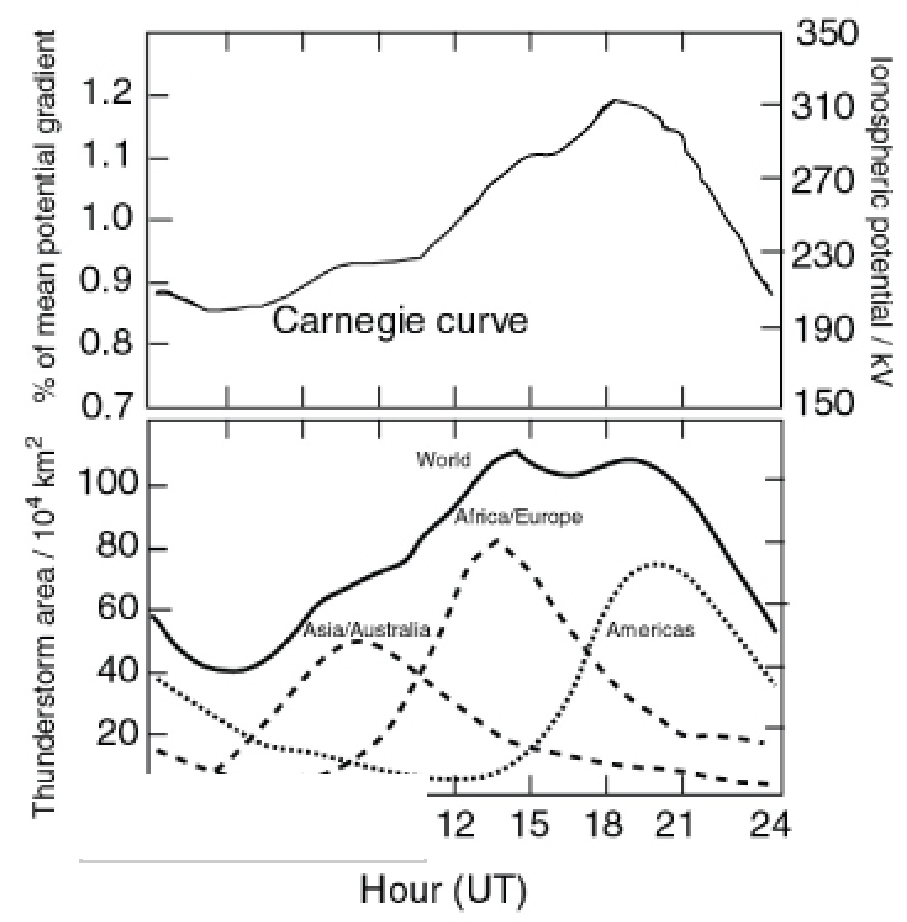
\includegraphics[scale=.6]{GEC/Figures/Carnegie_Curve.pdf} 
   \caption{
   Ionospheric potential and thunderstorm area again universal time showing the traditional Carnegie curve.
   Adapted from \citet{Whipple1936}}
   \label{gec:fig:Carnegie}
\end{figure}

The global electric circuit is the geoelectric system linking the source and discharge mechanism of the electric potential between the Earth and the ionosphere.
The Earth and the ionosphere form a large spherical capacitor charged to $\sim$250 kV with the atmosphere acting as the insulator between the two.
While air has a high resistivity the large surface area of the Earth results in a fairly low resistance between the ionosphere and ground, this low resistance allows for the ionosphere to discharge over fair weather regions resulting in the global fair weather return current.
On the other side of the circuit are thunderstorms acting as sources to constantly charge the ionosphere, without a constance source the system would discharge in $\sim$10 minutes \citep{Volland1984}.
It is still debated which components of thunderstorms act as the primary source of the circuit and whether there are other contributors to the circuit.

\subsubsection*{Why Study the Global Electric Circuit?}

Recent research on the global electric circuit is suggestive that the fair weather return current plays an important role in cloud microphysics and climate.
Specifically in the scavenging of cloud condensation and ice-forming nuclei \citep{Tinsley2007}.
The effects on the scavenging rates have a broader impact on precipitation rates, cloud cover, and possibly regional climate. 
 
\citet{Kniveton2004} shows how a decrease in the galactic cosmic ray flux was associated with negative cloud anomalies, while in \citet{Siingh2007} the return current is discussed as the intermediary between solar activity and climatic effects.
Further, \citet{Kniveton2008} studied how variations in the fair weather electric field relate to cloud cover and tentatively posits that solar activity could have an effect of global climate through the fair weather return current.
However they state that a better measure of the global return current would be needed to confidently study that theory.
 
One result of the proposed work is the possibility of using global lightning or thunderstorm activity as a direct proxy for measuring the fair weather return current, allowing further study into the relation between solar activity and climate.

Other research and models have suggested that lightning and thunderstorm activity are either not major contributors or not the only significant contributor to the circuit \citep{Rycroft2008,Liu2010}.
In these cases the major contributor is precipitation from not just thunderstorms but also electrified clouds.
By attempting to link global lightning or thunderstorm activity to the measured return current we plan to test the theories suggesting other contributors play a significant role.

\subsubsection*{Time Averaging}

An obstacle in determining the source function of the global electric circuit is the necessity of many measurement techniques to average data over long spans of time.
In some cases this is necessary to eliminate effects due to the local environment and other times it is done so that they data resembles the well known Carnegie curve.
One unexplained observation made by \citet{Holzworth1984} is of the vertical fair weather return current varying by a factor of two while the Carnegie curve has variations of $\pm20$\% \citep{Whipple1929}.
It is one of the goals of this proposed work to examine the relation between two potential sources of the circuit and the return current in high time resolution in order to explain the large daily deviations away from the normal Carnegie curve.

\subsubsection*{Recent Research}

Most of the recent experimental research on the global circuit has involved making measurements of the system using either ground based or satellite measurements.
Schumann resonances have been used as a method for measuring lightning activity as the source function, however the measurements tend to suffer from large day-night terminator effects \citep{Price2007} as well as being a modal phenomena.
A more direct measure of the circuit are field-mill measurements, \citet{Burns2005} used field mill data from Vostok, Antarctica to study interannual variations in the fields.
It is explained how the data needed to be corrected for the dawn-to-dusk electric potential which acts as a secondary generator in polar regions.
Despite the high time resolution of the field mill measurements the studies used a bimonthly average for the good days of data, similarly they removed any data which had large jumps in field values, one of the observed effects we want to investigate.
A more successful measurement was made by \citet{Holzworth1984} in which a balloon was tethered at 0.62km to measure the electric potential gradient.
They measured high daily variations of the gradient and their long term averages matched the carnegie curve, for this method static build up on instruments and current leakages were large factors in the uncertainty.

There has been one study by \citet{Holzworth2005} in which the return current results from the stratospheric Polar Patrol Balloon (PPB) campaign in 2003 was compared to the lightning activity of the nascent World Wide Lightning Location Network (WWLLN, see http://wwlln.net).
Here they showed how lightning activity and return current variations matched, however they could not prove anything conclusively about the source function as the network had poor coverage at the time and the global detection efficiency was unknown.

\subsubsection*{WWLLN}

The World Wide Lightning Location Network determines the location for nearly all lightning producing storms around the globe in real time \citep{Jacobson2006c}.
The network uses 57 Very Low Frequency (VLF) radio wave receivers distributed around the globe to identify the time of group arrival  for the wave packets of individual lightning sferics \citep{Dowden2002d}.
As stations are added the accuracy and detection efficiency of the network improves, as of 2010 the network located most strokes to within 10 kilometers and $<$10 $\mu$s with an estimated detection efficiency of about 11\% for all strokes and $>$30\% for more powerful strokes \citep{Abarca2010,Rodger2009}.
WWLLN lightning location data have recently been used for advances in space science \citep{Kumar2009,Holzworth2011}, meteorology \citep{Price2009,Thomas2010d}, and detailed lightning physics \citep{Connaughton2010a} to name a few. 

Recently the capability to estimate the absolute peak current of return strokes along with the VLF far-field RMS power of the strokes has been added to WWLLN \citep{Hutchins2011}.
This has enabled dynamic global detection efficiency maps of the network which will be used in generating the global circuit source function.

\subsubsection*{Proposed Flights}

This proposal requests support for a set of stratospheric balloons to be flown over the ocean in fair weather conditions while simultaneous measures of global lightning activity are made by the World Wide Lightning Location Network.
We have a proven capability for designing, fabricating and launching stratospheric balloons \citep{Holzworth2005,Thomas2004,Holzworth1985}, we also develop, operate and run WWLLN (see above).
The recent improvements to WWLLN have enabled the network to measure the far-field radiated power of detected strokes as well as the relative and absolute detection efficiencies of the network, allowing it to predict the total lightning activity contributing to the global circuit \citep{Hutchins2011}.
We will base the design of the payloads on the proven design flown in the (nsf funded?) [CAMPAIGN] with improvements and changes explained in the Technical Description section below.
%In addition to the in situ measurement and the long range lightning network we will also make a set of supplemental ground based measurements to help with the analysis of the other data CITE/COLLABORATION
The proposed balloon campaign will launch two balloons out of Oregon over the Pacific Ocean for a three week campaign during the months of January and February, determined to be the best time for fair weather measurements with balloons [Citation?]

\subsection*{Theory}

The study of the global electric circuit can broadly be divided into two categories, studies of the fair weather return current and studies of the source function.
Studies of the return current focuses on conductivity \citep{Rycroft2008}, solar effects on the system \citep{Tinsley2007}, and how the return current effects weather and climate \citep{Kniveton2008}.
Source studies are mainly models or highly averaged data sets attempting to match the proposed source to either the Carnegie curve or climatic variables \citep{Liu2010}.

\subsubsection*{Return Current}

Depending on the type of measurement used atmospheric conductivity is often only used in determining the return current in conjunction with electric field measurements, however some recent studies \citep{Rycroft2008} have stressed the importance of conductivity in understanding the system.
Discussions of conductivity show that it possibly plays an important role in determining the return current and that the uneven distribution of atmospheric conductivity around the globe can contribute to the return current.

%Similarly the dawn-to-dusk electric fields at the polar cap can act as generators which effect the vertical return current.

The effects of the Sun on the atmosphere can also possibly  play an important role in the global electric circuit.
Solar energetic particles and electron precipitation could drive part of the global circuit or have direct effects on regional conductivity in the system \citep{Tinsley2007}.
Indirectly the Sun modulates the flux of galactic cosmic rays which effect the global conductivity and return current. some suggest that the return current has an effect on cloud cover, temperature, surface pressure and winter cyclones \citep{Kniveton2008,Tinsley2007}.

\subsubsection*{Source Function}

Several different theories regarding the return current have been discussed, the source function of the global circuit is a more debated topic.
Cloud to ground lightning has long been considered the source for the global electric circuit with the strokes acting as the pumping mechanism to charge the tops of thunderclouds \citep{Roble1986}.
It was estimated by \citet{Wait1960} that a single 3-km long return stroke of 1000kA will charge the ionosphere by 1V, and the continual global lightning then maintains the ionospheric potential.
A model of \citet{Anderson1969} shows that just the pumping action of lightning can maintain the potential, but there have been some doubts about these models \citep{Hill1971}.
It is possible for lightning strokes to be the main driver though some measurements show that the return current varies too slowly to be charged by an impulsive source \citep{Krider1982}.

\citet{Rycroft2008} claims that the effects of lightning, through sferics and Schumann Resonances, solely impact the AC component of the global circuit, that is the part within the Earth-Ionosphere waveguide.
The AC component of the circuit is then separate from the DC component which includes the return current.
While some models may suggest this the high time resolution study proposed here will directly address this model.

Aside from lightning an alternative source of the global circuit is the precipitation from thunderstorms and possibly electrified clouds.
The idea being that the charged rain and ice carry charge from the cloud and drive the global circuit \citep{Rycroft2008}.
\citet{Liu2010} used average precipitation rates and thunderstorm data from the Tropical Rainfall Measuring Mission (TRMM) satellite to show that thunderstorm and electrified cloud activity can be matched to the Carnegie curve.
However it may be that the cloud to ground lightning within those clouds actually drive the circuit with the precipitation rates serving as proxy measurements for lightning activity.
Since WWLLN detects 99\% of thunderstorms along with the stroke rates it will be possible to test both thunderstorm activity and stroke activity as drivers for the measured return current \citep{Jacobson2006c}.

%\subsubsection*{Measurement - Both for Validation}
%
%Until recently it has not been feasible to make direct measures of both source and sink of the global circuit, though there have been studies utilizing proxy measurements for either one or both components CITE CITE. CITE used METHOD and found that RESULT, suggestion that RESULT2. This lends support to the idea that lightning is the primary driver of the electric circuit but possibly not the sole contributor.
%
%What is lacking for validating/refuting said theories.
%
%Measurements needed for each of the models or what they are lacking.
%
%Describe past measurements supporting/refuting the differing theories.
%
%Mention there is a lack of good measurement for all of the theories which is what we are doing.
%
%\subsubsection*{Measurement - Balloon}
%
%How the balloon will measure the relevant parts of Jz and other components thought to have an effect.
%
%\subsubsection*{Measurement - WWLLN}
%
%How WWLLN measure the stroke count, peak current, power radiated, total global thunderstorms. Also will have detection efficiency corrections to give global estimates.


\subsection*{Scientific Objectives}

With the recent upgrades to the WWLLN it is now possible for the first time to measure both the source of the global circuit and the fair weather return current in high time resolution.
With the lightning network already in place, we propose to conduct a balloon campaign with the following objectives:

\begin{enumerate}
\item{\underline{Primary Objective:} Measure the fair weather return current in high time resolution over the course of several weeks.}
\item{\underline{Secondary Objectives:}
\begin{enumerate}
\item{Generate and validate WWLLN derived global circuit source functions.}
\item{Compare lightning and thunderstorm activity to return current in high time resolution to test competing theories of global circuit sources.}
\item{Examine the contribution of galactic cosmic ray flux to variations of the return current.}
\item{Establish lightning activity as a proxy for the fair weather return current.}
\end{enumerate}}
\end{enumerate}

\subsection*{Technical Objectives}

\begin{enumerate}
\item{Fabricate and calibrate [SENSORS] for 3 high altitude balloon payloads.}
\item{Launch the balloons over the Pacific a week apart to ensure separation of ~1000km.}
\item{Measure the fair weather electric field, atmospheric conductivity, and x-ray flux from the balloons and simultaneous ground measurements of lightning activity and galactic cosmic ray flux.}
\item{Analyze the data from the balloon campaigns in relation to the ground based measurements to perform a detailed study of the contribution of lightning and thunderstorm activity to the global electric circuit.}
\item{Report on the findings and conclusions through scientific meetings, workshops, and publications.}
\end{enumerate}

\subsection*{Anticipated Results}

It is anticipated that the fair weather return current from the balloon will match the WWLLN data after being corrected for detection efficiency.
Depending on the actual source function the current will match to the stroke rate, total peak current or thunderstorm activity.
It is expected that the WWLLN results may not fully match the return current as there might be other contributors to the return current such as solar modulation.
If that is the case it should manifest itself as a small modulation on top of the signal attributed to the measurements made by WWLLN.
By simultaneously measuring the galactoc cosmic ray flux/[Other sensors] we plan to be able to account for the modulation.